\documentclass[12pt, twoside]{book}

% variable values
\input variables.tex

\ifshowframe{}
    \usepackage[a4paper,top=2.5cm,bottom=2.5cm,left=3.5cm,right=2cm,showframe]{geometry}
\else
    \usepackage[a4paper,top=2.5cm,bottom=2.5cm,left=3.5cm,right=2cm]{geometry}
\fi
\usepackage{microtype}
\usepackage[slovak,USenglish]{babel}
\usepackage[utf8]{inputenc}
\usepackage[T1]{fontenc}

\linespread{1.25} % this means 1.5 line spacing

% more package imports and custom commands
\input definitions.tex

\begin{document}

\ifenglish{}
    \selectlanguage{USenglish}
\else
    \selectlanguage{slovak}
\fi

\frontmatter
\pagenumbering{gobble}

% COVER
\thispagestyle{empty}

{
    \sc\large

    \begin{center}
        \thesisuniversity{}\\
        \thesisfaculty{}

        \vfill

        \iflogoFMFI{}
            \begin{figure}[!hbt]
                \centering
                
\includegraphics[width=0.4\textwidth]{images/logoFMFI.pdf}
            \end{figure}
        \fi

        {\LARGE\thesisname}\\
        \thesistype{}
    \end{center}

    \vfill

    \noindent
    \thesisyear{}\\
    \thesisauthor{}
}

\cleardoublepage{}

% TITLE PAGE
\frontmatter
\thispagestyle{empty}

\begin{center}
    \sc\large
    \thesisuniversity{}\\
    \thesisfaculty{}

    \vfill

    \iflogoFMFI{}
        \begin{figure}[!hbt]
            \centering
            
\includegraphics[width=0.4\textwidth]{images/logoFMFI.pdf}
        \end{figure}
    \fi

    {\LARGE\thesisname}\\
    \thesistype{}
\end{center}

\vfill

\noindent
\begin{tabular}{ll}
    \ifenglish{}Study Programme:\else{}Študijný program:   \fi & \thesisprogramme{}\\
    \ifenglish{}Field of Study: \else{}Študijný odbor:     \fi & \thesisfield{}\\
    \ifenglish{}Department:     \else{}Školiace pracovisko:\fi & \thesisdepartment{}\\
    \ifenglish{}Supervisor:     \else{}Školiteľ:           \fi & \thesissupervisor{}\\
    \ifconsultant{}\ifenglish{}Consultant:\else{}Konzultant:\fi & \thesisconsultant{}\\ \fi
\end{tabular}

\vfill

\noindent
\thesislocation, \thesisyear{}\\
\thesisauthor{}

\cleardoublepage{}

% ASSIGNMENT
\newpage
\thispagestyle{empty}

\noindent
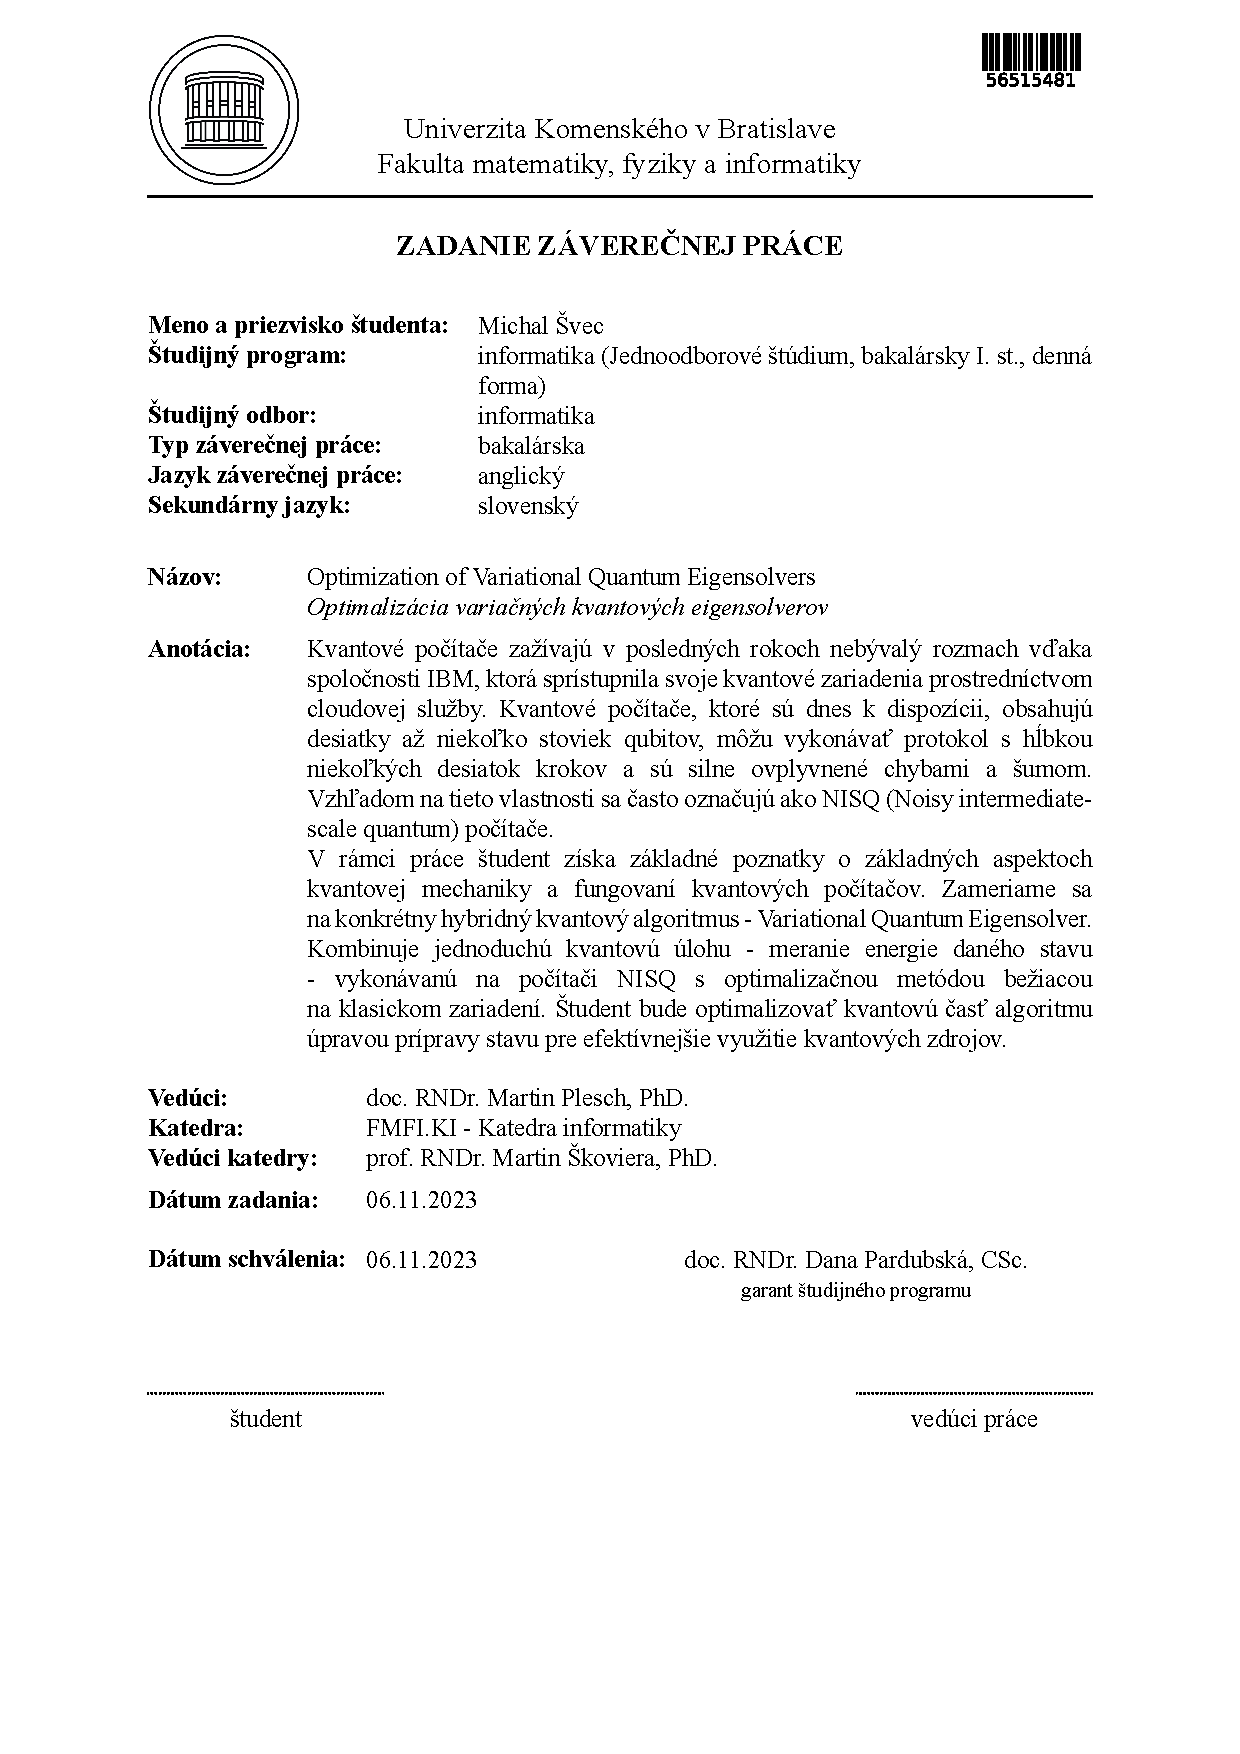
\includegraphics[trim=2.5cm 5cm 2.5cm 0,width=\textwidth]{images/assignment-sk.pdf}

\ifenglish{}
    \newpage
    \thispagestyle{empty}

    \noindent
    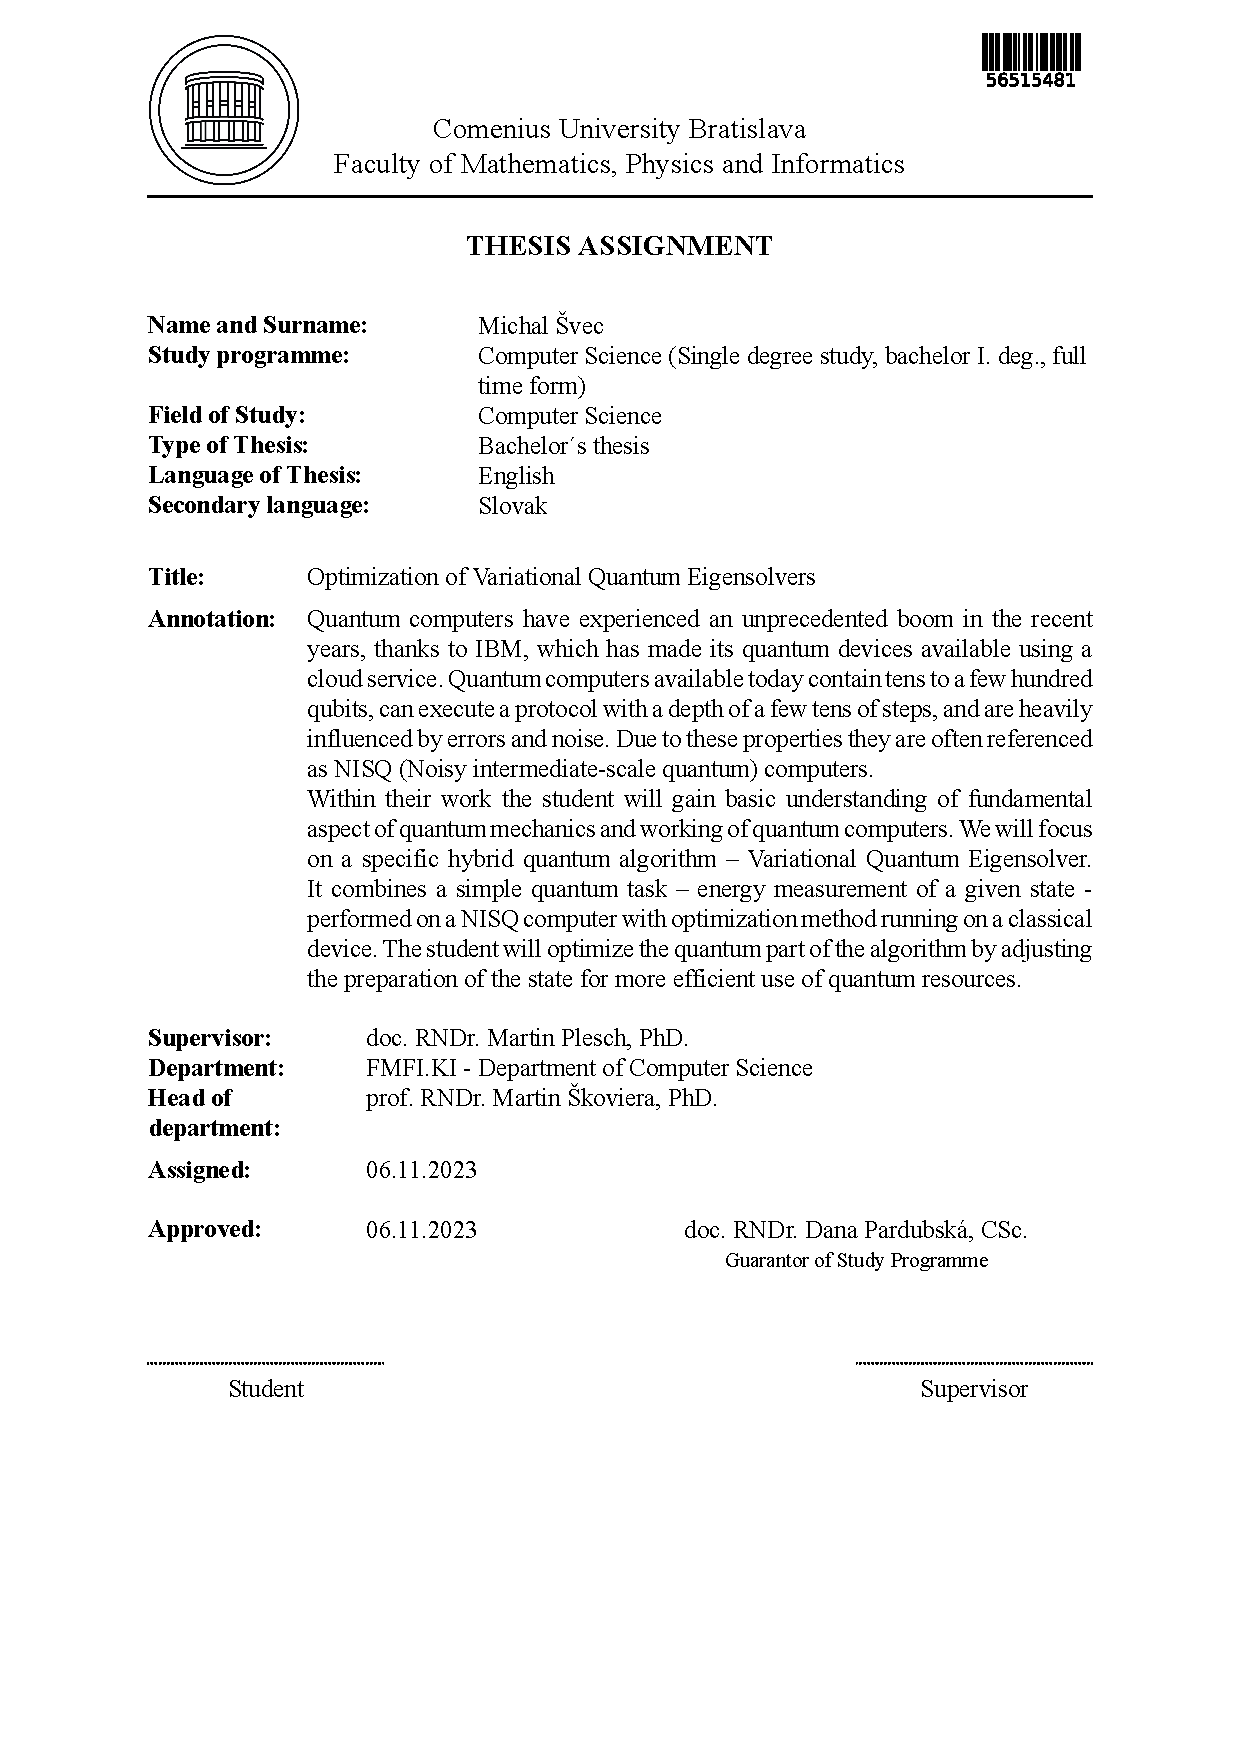
\includegraphics[trim=2.5cm 5cm 2.5cm 0,width=\textwidth]{images/assignment-en.pdf}
\fi

% ACKNOWLEDGEMENTS
\newpage

~\vfill
\paragraph*{\ifenglish{}Acknowledgments:\else{}Poďakovanie:\fi} \thesisacknowledgments{}

% ABSTRACT SK
\newpage

\begin{otherlanguage}{slovak}
    \section*{Abstrakt}

    \thesisabstractsk{}

    \paragraph*{Kľúčové slová:} \thesiskeywordssk{}
\end{otherlanguage}

% ABSTRACT EN
\newpage

\begin{otherlanguage}{USenglish}
    \section*{Abstract}

    \thesisabstracten{}

    \paragraph*{Keywords:} \thesiskeywordsen{}
\end{otherlanguage}

% TABLE OF CONTENTS, LIST OF FIGURES
\newpage
\tableofcontents

\newpage
\listoffigures

% CONTENTS
\mainmatter{}
\thesischapters{}

% BIBLIOGRAPHY
\newpage
\thispagestyle{empty}

\bibliographystyle{unsrt}
\bibliography{references}

% APPENDICES
\appendix
\thesisappendices{}

\end{document}
